%%%%%%%%%%%%%%%%%%%%%%%%%%%%%% Preamble
\documentclass{article}
\usepackage{amsmath,amssymb,amsthm,fullpage}
\usepackage[a4paper,bindingoffset=0in,left=1in,right=1in,top=1in,
bottom=1in,footskip=0in]{geometry}
\newtheorem*{prop}{Proposition}
%\newcounter{Examplecount}
%\setcounter{Examplecount}{0}
\newenvironment{discussion}{\noindent Discussion.}{}
\setlength{\headheight}{12pt}
\setlength{\headsep}{10pt}
\usepackage{listings}
\usepackage{graphicx}
\usepackage{fancyhdr}
\graphicspath{{images/}}

\newcommand*{\wb}{\ensuremath{\mathbf{w}}}
\newcommand*{\yb}{\ensuremath{\mathbf{y}}}
\newcommand*{\Xb}{\ensuremath{\mathbf{X}}}
\newcommand*{\Ib}{\ensuremath{\mathbf{I}}}
\pagestyle{fancy}
\fancyhf{}
\lhead{CS155 Homework 1}
\rhead{Matt Lim}
\begin{document}
%%%%%%%%%%%%%%%%%%%%%%%%%%%%%% Problem 1
\section*{Problem 1}

\subsection*{Question A}
Adding the penalty term cannot decrease the training (in-sample) error. This
is because adding the penalty term is equivalent to constraining the model
complexity. And constraining the model complexity must either harm the in-sample
error or keep it the same; we cannot bring the in sample error \textit{down}
by constraining which models we use.

Adding the penalty term does not always decrease the out-of-sample errors. We
can find that it does not decrease the out-of-sample errors
in cases when adding the penalty term causes underfitting; that is, when
it causes a simpler model to be used to model a more complex one. Basically,
adding the penalty term can be harmful or unhelpful when a more complex
model generalizes better than a simpler model.

\subsection*{Question B}
We rarely use $\ell_0$ regularization because it involves the $\ell_0$ norm of
$\wb$. And the $\ell_0$ norm of $\wb$ is not continuous (by its definition),
which means we cannot perform gradient descent (because we can't find the gradient
or sub gradient of the regularization penalty term).

\subsection*{Question C}
\begin{figure}[h]
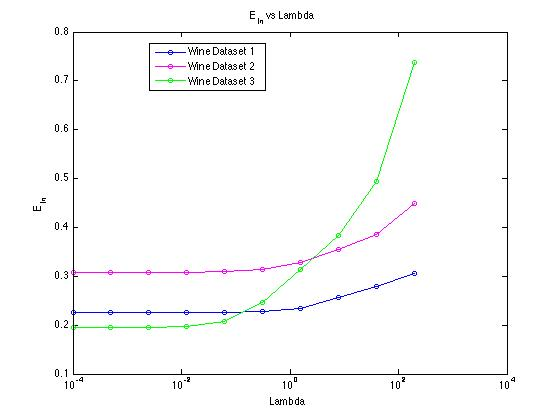
\includegraphics[width=16cm]{e_in}
\end{figure}
\begin{figure}[p]
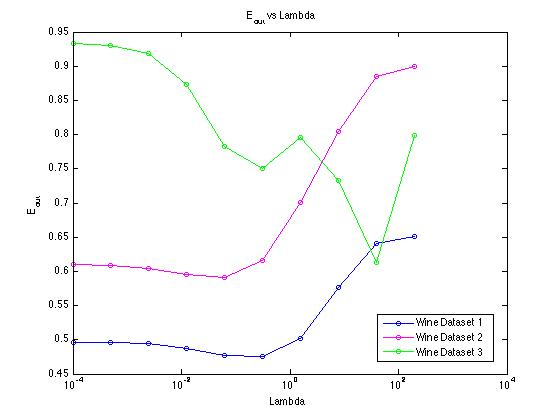
\includegraphics[width=16cm]{e_out}
\vspace{5mm}
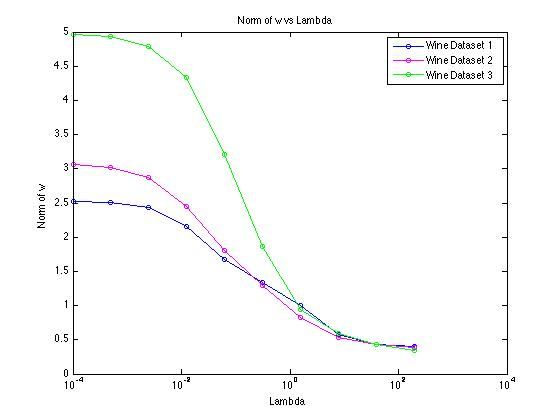
\includegraphics[width=16cm]{w_norm}
\end{figure}
\clearpage

\subsection*{Question D}
\begin{description}
    \item[training]
        For lower lambdas, training with Wine Dataset 3 gives us slightly
        lower $E_{in}$, but for higher lambdas, training with Wine Dataset 1 gives us
        much lower $E_{in}$ as training with Wine Dataset 3 gets much worse.
        This means more complex models are better at fitting Dataset 3 and
        simpler models are worse at fitting Dataset 3. The former can be explained
        by the following reason. Since Dataset 3 is a smaller subset of Dataset 1,
        it is easier to more closely fit all the points with a more complex model.
        This makes sense; it is easier to fit less points than more points with
        more complex models.
        The latter can be explained by the following reason. Since Dataset 3
        is a smaller subset of Dataset 1, when the models get simpler and fit
        the data less closely, points with large error negatively affect the
        overall $E_{in}$ much more for Dataset 3 than Dataset 1 (again, because
        Dataset 3 is a smaller subset of Dataset 1).
    \item[validation]
        For basically all lambdas, training with Wine Dataset 1 gives us lower
        $E_{out}$, except for at $\lambda = 39.0625$, where training with
        Wine Dataset 3 gives us a slightly lower $E_{out}$. We can explain this
        trend with the fact that variance should be lower when training with
        Wine Dataset 1 and with equivalent lambdas, because at equivalent
        lambdas model complexity is the same, but Wine Dataset 1 has more
        data points which reduces variance. Also, bias should be about the same
        whether training with Dataset 1 or 3 (keeping lambda constant),
        because bias only depends on model complexity and is independent of
        training data size. Thus, since the biases are around the same and
        the variance is lower when training with Dataset 1, by the
        Bias-Variance Decomposition, $E_{out}$ should be lower when training
        with Dataset 1.
\end{description}

\subsection*{Question E}
Around the midway point and going left, we start to see overfitting. We see
this as $E_{out}$
rises from its local minimum as lambda decreases (going left). This is overfitting
because we are increasing model complexity at the cost of hurting generalization
($\lambda$ is decreasing, $E_{out}$ is increasing).
Around the midway point and going right, we also start to see underfitting. We see
this as $E_{out}$ rises from its local minimum as lambda increases (going right).
This is underfitting because in this area, we are decreasing model complexity
and using models that are too constrained/simple and thus
cannot capture the data accurately enough, which is reflected in the
rising $E_{out}$ and $E_{in}$.

\subsection*{Question F}
We can see that the norm of $\wb$ decreases as $\lambda$ increases when we train
with Wine Dataset 1. This is because setting $\lambda$ to some value effectively
constrains the norm of $\wb$ to be less than or equal to some constant $c$. And
as $\lambda$ increases, the $c$ we are constraining the norm of $\wb$ to be
less than or equal to decreases. This intuitively makes sense, as we are trying
to minimize $E$, which contains the term $\frac{\lambda}{N}\wb^{\intercal}\wb$,
so as $\lambda$ increases bigger $\wb$s get more and more harmful. So basically,
the norm of $\wb$ decreases as $\lambda$ increases because a bigger $\lambda$
corresponds to a stricter constraint on the norm of $\wb$
(a smaller $c$ in $\wb^{\intercal}\wb \leq c$).

\subsection*{Question G}
I would choose $\lambda = 39.0625$  to train my final model, because it has
the lowest $E_{out}$ and thus has the best chance of generalizing out of sample.

\newpage
%%%%%%%%%%%%%%%%%%%%%%%%%%%%%% Problem 2
\section*{Problem 2}
\subsection*{Question A}
\subsubsection*{(1)}
Using Bayes rule and the given prior, we have that
\[ p(\wb|\mathcal{D}) = \frac{p(\mathcal{D}|\wb)p(\wb|\lambda)}
    {p(\mathcal{D})} \]
We start with
\[ \hat{\wb} = \underset{\wb}{\text{argmax}} \> p(\wb|\mathcal{D}) \]
We can now plug in the numerator of the first equation we wrote, excluding the
denominator as it does not have $\wb$ in it and we are maximizing over $\wb$.
\[ \hat{\wb} = \underset{\wb}{\text{argmax}} \> p(\mathcal{D}|\wb)
    p(\wb|\lambda) \]
\[ \hat{\wb} = \underset{\wb}{\text{argmax}} \>
    p(\mathcal{D}|\wb) \prod_{j=1}^{D} \frac{\lambda}{2} e^{-\lambda |w_j|} \]
We can now do the following:
\[ \hat{\wb} = \underset{\wb}{\text{argmax}} \>
    \log \Big(p(\mathcal{D}|\wb) \prod_{j=1}^{D} \frac{\lambda}{2}
    e^{-\lambda |w_j|} \Big) \]
because the quantity inside is nonnegative and log is monotonically
increasing so if you maximize it you maximize its argument. Then clearly we can just
minimize the negative to get the following.
\[ \hat{\wb} = \underset{\wb}{\text{argmin}} \>
    -\log \Big(p(\mathcal{D}|\wb)
    \prod_{j=1}^{D} \frac{\lambda}{2} e^{-\lambda |w_j|} \Big) \]
Now we can just apply log rules to get the following.
\[ \hat{\wb} = \underset{\wb}{\text{argmin}} \>
    - \Big( \log p(\mathcal{D}|\wb)
    + \log \prod_{j=1}^{D} \frac{\lambda}{2} e^{-\lambda |w_j|} \Big) \]
\[ \hat{\wb} = \underset{\wb}{\text{argmin}} \>
    - \Big( \log p(\mathcal{D}|\wb)
    + \sum_{j=1}^D \log \frac{\lambda}{2} e^{-\lambda |w_j|} \Big) \]
\[ \hat{\wb} = \underset{\wb}{\text{argmin}} \>
    - \Big( \log p(\mathcal{D}|\wb)
    + \sum_{j=1}^D \log \frac{\lambda}{2} + \log e^{-\lambda |w_j|} \Big) \]
We can get rid of all the $\log \frac{\lambda}{2}$ terms, as these are constant
with respect to $\wb$. This leaves us with
\[ \hat{\wb} = \underset{\wb}{\text{argmin}} \>
    - \Big( \log p(\mathcal{D}|\wb)
    + \sum_{j=1}^D \log e^{-\lambda |w_j|} \Big) \]
\[ \hat{\wb} = \underset{\wb}{\text{argmin}} \>
    - \Big( \log p(\mathcal{D}|\wb)
    + \sum_{j=1}^D -\lambda |w_j| \Big) \]
\[ \hat{\wb} = \underset{\wb}{\text{argmin}} \>
    - \log p(\mathcal{D}|\wb) + \lambda ||\wb||_1 \]

\subsubsection*{(2)}
Using Bayes rule and the given prior, we have that
\[ p(\wb|\mathcal{D}) = \frac{p(\mathcal{D}|\wb)
    p(\wb|\lambda)}{p(\mathcal{D})} \]
We start with
\[ \hat{\wb} = \underset{\wb}{\text{argmax}} \> p(\wb|\mathcal{D}) \]
We can now plug in the numerator of the first equation we wrote, excluding the
denominator as it does not have $\wb$ in it and we are maximizing over $\wb$.
\[ \hat{\wb} = \underset{\wb}{\text{argmax}} \> p(\mathcal{D}|\wb)
    p(\wb|\lambda) \]
\[ \hat{\wb} = \underset{\wb}{\text{argmax}} \>
    p(\mathcal{D}|\wb) \prod_{j=1}^{D}
    \sqrt{\frac{\lambda}{\pi}} e^{-\lambda w_j^2} \]
We can now do the following:
\[ \hat{\wb} = \underset{\wb}{\text{argmax}} \>
    \log \Big(p(\mathcal{D}|\wb)
    \prod_{j=1}^{D} \sqrt{\frac{\lambda}{\pi}} e^{-\lambda w_j^2} \Big) \]
because the quantity inside is nonnegative and log is monotonically
increasing so if you maximize it you maximize its argument. Then clearly we can just
minimize the negative to get the following.
\[ \hat{\wb} = \underset{\wb}{\text{argmin}} \>
    -\log \Big(p(\mathcal{D}|\wb)
    \prod_{j=1}^{D} \sqrt{\frac{\lambda}{\pi}} e^{-\lambda w_j^2} \Big) \]
Now we can just apply log rules to get the following.
\[ \hat{\wb} = \underset{\wb}{\text{argmin}} \>
    - \Big( \log p(\mathcal{D}|\wb)
    + \log \prod_{j=1}^{D} \sqrt{\frac{\lambda}{\pi}} e^{-\lambda w_j^2} \Big) \]
\[ \hat{\wb} = \underset{\wb}{\text{argmin}} \>
    - \Big( \log p(\mathcal{D}|\wb)
    + \sum_{j=1}^D \log \sqrt{\frac{\lambda}{\pi}} e^{-\lambda w_j^2} \Big) \]
\[ \hat{\wb} = \underset{\wb}{\text{argmin}} \>
    - \Big( \log p(\mathcal{D}|\wb)
    + \sum_{j=1}^D \log \sqrt{\frac{\lambda}{\pi}} + \log e^{-\lambda w_j^2} \Big) \]
We can get rid of all the $\log \sqrt{\frac{\lambda}{\pi}}$ terms, as these are
constant with respect to $\wb$. This leaves us with
\[ \hat{\wb} = \underset{\wb}{\text{argmin}} \>
    - \Big( \log p(\mathcal{D}|\wb)
    + \sum_{j=1}^D \log e^{-\lambda w_j^2} \Big) \]
\[ \hat{\wb} = \underset{\wb}{\text{argmin}} \>
    - \Big( \log p(\mathcal{D}|\wb)
    + \sum_{j=1}^D -\lambda w_j^2 \Big) \]
\[ \hat{\wb} = \underset{\wb}{\text{argmin}} \>
    - \log p(\mathcal{D}|\wb) + \lambda ||\wb||_2^2 \]

\subsubsection*{(3)}
We have that
\[ \yb \sim \mathcal{N}(\Xb \wb, \sigma^2 \Ib), \> \mathcal{D} \text{ contains }
    \Xb \text{ and } \yb \]
We start with
\[ \hat{\wb} = \underset{\wb}{\text{argmax}} \> p(\mathcal{D}|\wb) \]
The multivariate normal distribution has a density given by
the following when the second parameter ($\sigma^2 \Ib$ in our case) is positive
definite:
\[ \frac{1}{\sqrt{(2 \pi)^n |\sigma^2 \Ib|}}
    e^{-\frac{1}{2}(\yb - \Xb \wb)^{\intercal} (\sigma^2 \Ib)^{-1}(\yb - \Xb \wb)} \]
where $n$ is the number of training points.
Since $\sigma^2 \Ib$ is positive definite, we can use this density function.
This density function describes the relative likelihood for generating the dataset
$\mathcal{D}$ given a certain weight vector $\wb$. In other words, it is equivalent
to $p(\mathcal{D}|\wb)$. So we can plug it into the above equation to get the
following:
\[ \hat{\wb} = \underset{\wb}{\text{argmax}} \>
    \frac{1}{\sqrt{(2 \pi)^n |\sigma^2 \Ib|}}
    e^{-\frac{1}{2}(\yb - \Xb \wb)^{\intercal} (\sigma^2 \Ib)^{-1}(\yb - \Xb \wb)} \]
We can drop constants (terms that do not involve $\wb$) to get the following:
\[ \hat{\wb} = \underset{\wb}{\text{argmax}} \>
    e^{-\frac{1}{2}(\yb - \Xb \wb)^{\intercal} (\sigma^2 \Ib)^{-1}(\yb - \Xb \wb)} \]
We can now do the following:
\[ \hat{\wb} = \underset{\wb}{\text{argmax}} \>
    \log \Big( e^{-\frac{1}{2}(\yb - \Xb \wb)^{\intercal}
    (\sigma^2 \Ib)^{-1}(\yb - \Xb \wb)} \Big) \]
\[ \hat{\wb} = \underset{\wb}{\text{argmax}} \>
    -\frac{1}{2}(\yb - \Xb \wb)^{\intercal} (\sigma^2 \Ib)^{-1}(\yb - \Xb \wb) \]
because the quantity inside is nonnegative and log is monotonically
increasing so if you maximize it you maximize its argument. Then clearly we can just
minimize the negative (and get rid of constants) to get the following.
\[ \hat{\wb} = \underset{\wb}{\text{argmin}} \>
    (\yb - \Xb \wb)^{\intercal}(\yb - \Xb \wb) \]
\[ \hat{\wb} = \underset{\wb}{\text{argmin}} \> ||\yb - \Xb \wb||^2_2 \]

\subsection*{Question B}
\begin{figure}[p]
\caption{A plot of the each of the weights as a function of $\lambda$, where
    $\wb$ was estimated using linear regression with Lasso regularization}
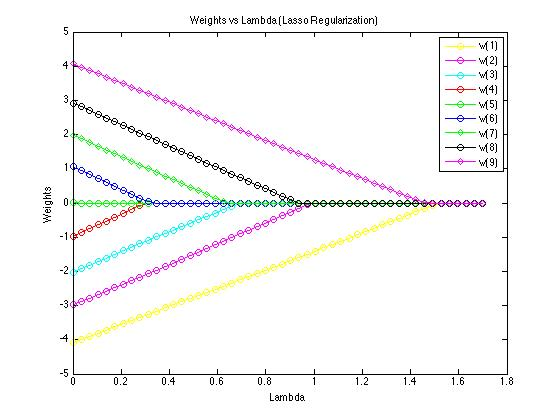
\includegraphics[width=14.8cm]{lasso_weights}
\caption{A plot of the each of the weights as a function of $\lambda$, where
    $\wb$ was estimated using linear regression with Ridge regularization}
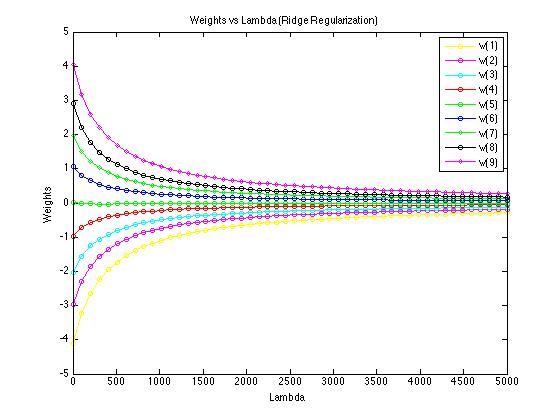
\includegraphics[width=14.8cm]{ridge_weights}
\end{figure}
\clearpage
\subsubsection*{(3)}
As the regularization parameter varies with Lasso regression, all the
estimated weights go to zero (before $\lambda = 1.8$).
As the regularization parameter varies with
Ridge regression, none of the estimated weights go to zero (at least up to
$\lambda = 50000$).
We can see the former behavior in the plot below:
\begin{figure}[h]
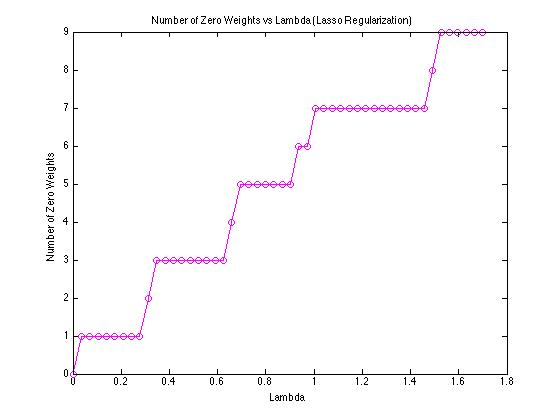
\includegraphics[width=15cm]{zeros}
\centering
\end{figure}

\subsection*{Question C}
Note: $\Xb$ is a matrix where each row is a single training point.
\subsubsection*{(1)}
We want to minimize over all the points, so we will minimize the following:
\[ f(\wb) = ||\yb - \Xb \wb||^2 + \lambda ||\wb||_1 \]
To minimize this, we can find the gradient
\[ \nabla f(\wb) = -2 \Xb^{\intercal}(\yb - \Xb \wb)
    + \frac{\lambda \wb}{|\wb|} \]
\[ \nabla f(\wb) = -2 \Xb^{\intercal}\yb + 2 \Xb^{\intercal} \Xb \wb
    \pm \lambda I \]
and set the gradient to $0$ (because $f$ is convex)
\[ -2 \Xb^{\intercal}\yb + 2 \Xb^{\intercal} \Xb \wb
    \pm \lambda I = 0 \]
\[ 2 \Xb^{\intercal} \Xb \wb = 2 \Xb^{\intercal}\yb \mp \lambda I \]
\[ \wb = (2 \Xb^{\intercal} \Xb)^{-1} (2 \Xb^{\intercal}\yb \mp \lambda I) \]

\subsubsection*{(2)}
We want to see if there exists a value for $\lambda$ such that
$\wb = 0$, and find the smallest such value.
From the above, we have that
\[ \wb = (2 \Xb^{\intercal} \Xb)^{-1} (2 \Xb^{\intercal}\yb \mp \lambda I) \]
We can see that we need the second term (involving $\lambda$ to equal $0$.
So we have that
\[ 0 = (2 \Xb^{\intercal}\yb \mp \lambda I) \]
Now we get two cases.
\[ \wb > 0 \implies 0 = 2 \Xb^{\intercal}\yb - \lambda I \implies
    \lambda = 2 \Xb^{\intercal}\yb \]
\[ \wb < 0 \implies 0 = 2 \Xb^{\intercal}\yb + \lambda I \implies
    \lambda = -2 \Xb^{\intercal}\yb \]
Notice that when $\wb < 0$, $\Xb^{\intercal} \yb < 0$ as well. We can see this
with the following reasoning.
\[ \wb = (2 \Xb^{\intercal} \Xb)^{-1} (2 \Xb^{\intercal}\yb + \lambda I) < 0 \]
\[ (2 \Xb^{\intercal}\yb + \lambda I) < 0 \implies \Xb^{\intercal} \yb < 0 \]
Therefore, the two cases above collapse into the one case below:
\[ \lambda = ||2 \Xb^{\intercal} \yb|| \]
This is the smallest such value.

\subsubsection*{(3)}
We want to minimize over all the points, so we will minimize the following:
\[ f(\wb) = ||\yb - \Xb \wb||^2 + \lambda||\wb||_1 \]
\[ f(\wb) = ||\Xb \wb - \yb||^2 + \lambda||\wb||_1 \]
To minimize this, we can find the gradient
\[ \nabla f(\wb) = 2 \Xb^{\intercal} (\Xb \wb - \yb) + 2 \lambda \wb \]
\[ \nabla f(\wb) = 2 \Xb^{\intercal} \Xb \wb - 2 \Xb^{\intercal} \yb
    + 2 \lambda \wb \]
and set the gradient to $0$ (because $f$ is convex)
\[ 2 \Xb^{\intercal} \Xb \wb - 2 \Xb^{\intercal} \yb
    + 2 \lambda \wb = 0 \]
\[ \Xb^{\intercal} \Xb \wb - \Xb^{\intercal} \yb + \lambda \wb = 0 \]
\[ (\Xb^{\intercal} \Xb + \lambda I) \wb = \Xb^{\intercal} \yb \]
\[ \wb = (\Xb^{\intercal} \Xb + \lambda I)^{-1} \Xb^{\intercal} \yb \]

\subsubsection*{(4)}
We want to see if there exists a value for $\lambda$ such that $\wb = 0$.
So basically, since
\[ \wb = (\Xb^{\intercal} \Xb + \lambda I)^{-1} \Xb^{\intercal} \yb \]
we want
\[ (\Xb^{\intercal} \Xb + \lambda I)^{-1} \Xb^{\intercal} \yb = 0 \]
\[ (\Xb^{\intercal} \Xb + \lambda I)^{-1} = 0 \]
But for this equality to hold, the inverse of some matrix would have to equal
0. But this is not possible (because $\mathbf{C}\mathbf{D} = \mathbf{D}\mathbf{C}
= I \neq 0$). So there does not exist a value for $\lambda$
such that $\wb = 0$.

\end{document}
